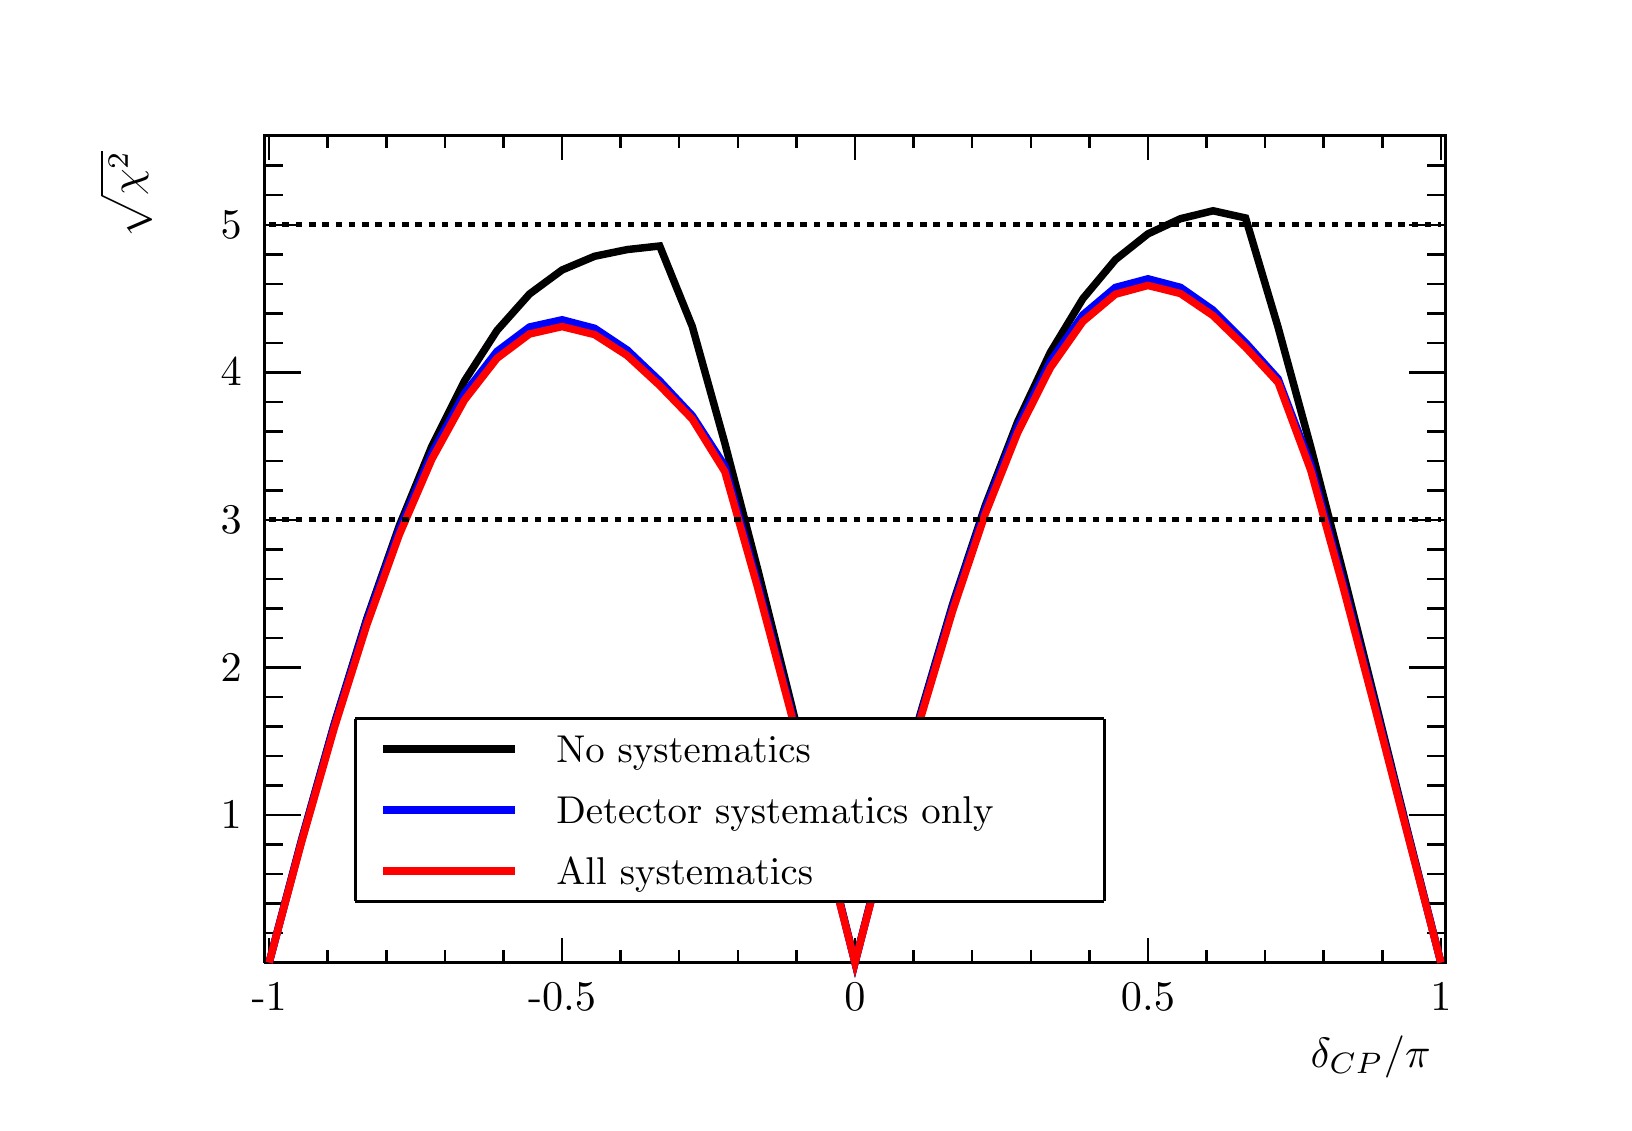
\begin{tikzpicture}
\pgfdeclareplotmark{cross} {
\pgfpathmoveto{\pgfpoint{-0.3\pgfplotmarksize}{\pgfplotmarksize}}
\pgfpathlineto{\pgfpoint{+0.3\pgfplotmarksize}{\pgfplotmarksize}}
\pgfpathlineto{\pgfpoint{+0.3\pgfplotmarksize}{0.3\pgfplotmarksize}}
\pgfpathlineto{\pgfpoint{+1\pgfplotmarksize}{0.3\pgfplotmarksize}}
\pgfpathlineto{\pgfpoint{+1\pgfplotmarksize}{-0.3\pgfplotmarksize}}
\pgfpathlineto{\pgfpoint{+0.3\pgfplotmarksize}{-0.3\pgfplotmarksize}}
\pgfpathlineto{\pgfpoint{+0.3\pgfplotmarksize}{-1.\pgfplotmarksize}}
\pgfpathlineto{\pgfpoint{-0.3\pgfplotmarksize}{-1.\pgfplotmarksize}}
\pgfpathlineto{\pgfpoint{-0.3\pgfplotmarksize}{-0.3\pgfplotmarksize}}
\pgfpathlineto{\pgfpoint{-1.\pgfplotmarksize}{-0.3\pgfplotmarksize}}
\pgfpathlineto{\pgfpoint{-1.\pgfplotmarksize}{0.3\pgfplotmarksize}}
\pgfpathlineto{\pgfpoint{-0.3\pgfplotmarksize}{0.3\pgfplotmarksize}}
\pgfpathclose
\pgfusepathqstroke
}
\pgfdeclareplotmark{cross*} {
\pgfpathmoveto{\pgfpoint{-0.3\pgfplotmarksize}{\pgfplotmarksize}}
\pgfpathlineto{\pgfpoint{+0.3\pgfplotmarksize}{\pgfplotmarksize}}
\pgfpathlineto{\pgfpoint{+0.3\pgfplotmarksize}{0.3\pgfplotmarksize}}
\pgfpathlineto{\pgfpoint{+1\pgfplotmarksize}{0.3\pgfplotmarksize}}
\pgfpathlineto{\pgfpoint{+1\pgfplotmarksize}{-0.3\pgfplotmarksize}}
\pgfpathlineto{\pgfpoint{+0.3\pgfplotmarksize}{-0.3\pgfplotmarksize}}
\pgfpathlineto{\pgfpoint{+0.3\pgfplotmarksize}{-1.\pgfplotmarksize}}
\pgfpathlineto{\pgfpoint{-0.3\pgfplotmarksize}{-1.\pgfplotmarksize}}
\pgfpathlineto{\pgfpoint{-0.3\pgfplotmarksize}{-0.3\pgfplotmarksize}}
\pgfpathlineto{\pgfpoint{-1.\pgfplotmarksize}{-0.3\pgfplotmarksize}}
\pgfpathlineto{\pgfpoint{-1.\pgfplotmarksize}{0.3\pgfplotmarksize}}
\pgfpathlineto{\pgfpoint{-0.3\pgfplotmarksize}{0.3\pgfplotmarksize}}
\pgfpathclose
\pgfusepathqfillstroke
}
\pgfdeclareplotmark{newstar} {
\pgfpathmoveto{\pgfqpoint{0pt}{\pgfplotmarksize}}
\pgfpathlineto{\pgfqpointpolar{44}{0.5\pgfplotmarksize}}
\pgfpathlineto{\pgfqpointpolar{18}{\pgfplotmarksize}}
\pgfpathlineto{\pgfqpointpolar{-20}{0.5\pgfplotmarksize}}
\pgfpathlineto{\pgfqpointpolar{-54}{\pgfplotmarksize}}
\pgfpathlineto{\pgfqpointpolar{-90}{0.5\pgfplotmarksize}}
\pgfpathlineto{\pgfqpointpolar{234}{\pgfplotmarksize}}
\pgfpathlineto{\pgfqpointpolar{198}{0.5\pgfplotmarksize}}
\pgfpathlineto{\pgfqpointpolar{162}{\pgfplotmarksize}}
\pgfpathlineto{\pgfqpointpolar{134}{0.5\pgfplotmarksize}}
\pgfpathclose
\pgfusepathqstroke
}
\pgfdeclareplotmark{newstar*} {
\pgfpathmoveto{\pgfqpoint{0pt}{\pgfplotmarksize}}
\pgfpathlineto{\pgfqpointpolar{44}{0.5\pgfplotmarksize}}
\pgfpathlineto{\pgfqpointpolar{18}{\pgfplotmarksize}}
\pgfpathlineto{\pgfqpointpolar{-20}{0.5\pgfplotmarksize}}
\pgfpathlineto{\pgfqpointpolar{-54}{\pgfplotmarksize}}
\pgfpathlineto{\pgfqpointpolar{-90}{0.5\pgfplotmarksize}}
\pgfpathlineto{\pgfqpointpolar{234}{\pgfplotmarksize}}
\pgfpathlineto{\pgfqpointpolar{198}{0.5\pgfplotmarksize}}
\pgfpathlineto{\pgfqpointpolar{162}{\pgfplotmarksize}}
\pgfpathlineto{\pgfqpointpolar{134}{0.5\pgfplotmarksize}}
\pgfpathclose
\pgfusepathqfillstroke
}
\definecolor{c}{rgb}{1,1,1};
\draw [color=c, fill=c] (0,0) rectangle (20,13.639);
\draw [color=c, fill=c] (3,1.77307) rectangle (18,12.2751);
\definecolor{c}{rgb}{0,0,0};
\draw [c,line width=0.9] (3,1.77307) -- (3,12.2751) -- (18,12.2751) -- (18,1.77307) -- (3,1.77307);
\definecolor{c}{rgb}{1,1,1};
\draw [color=c, fill=c] (3,1.77307) rectangle (18,12.2751);
\definecolor{c}{rgb}{0,0,0};
\draw [c,line width=0.9] (3,1.77307) -- (3,12.2751) -- (18,12.2751) -- (18,1.77307) -- (3,1.77307);
\draw [c,line width=0.9] (3,1.77307) -- (18,1.77307);
\draw [c,line width=0.9] (3.05952,2.07994) -- (3.05952,1.77307);
\draw [c,line width=0.9] (3.80357,1.9265) -- (3.80357,1.77307);
\draw [c,line width=0.9] (4.54762,1.9265) -- (4.54762,1.77307);
\draw [c,line width=0.9] (5.29167,1.9265) -- (5.29167,1.77307);
\draw [c,line width=0.9] (6.03571,1.9265) -- (6.03571,1.77307);
\draw [c,line width=0.9] (6.77976,2.07994) -- (6.77976,1.77307);
\draw [c,line width=0.9] (7.52381,1.9265) -- (7.52381,1.77307);
\draw [c,line width=0.9] (8.26786,1.9265) -- (8.26786,1.77307);
\draw [c,line width=0.9] (9.0119,1.9265) -- (9.0119,1.77307);
\draw [c,line width=0.9] (9.75595,1.9265) -- (9.75595,1.77307);
\draw [c,line width=0.9] (10.5,2.07994) -- (10.5,1.77307);
\draw [c,line width=0.9] (11.244,1.9265) -- (11.244,1.77307);
\draw [c,line width=0.9] (11.9881,1.9265) -- (11.9881,1.77307);
\draw [c,line width=0.9] (12.7321,1.9265) -- (12.7321,1.77307);
\draw [c,line width=0.9] (13.4762,1.9265) -- (13.4762,1.77307);
\draw [c,line width=0.9] (14.2202,2.07994) -- (14.2202,1.77307);
\draw [c,line width=0.9] (14.9643,1.9265) -- (14.9643,1.77307);
\draw [c,line width=0.9] (15.7083,1.9265) -- (15.7083,1.77307);
\draw [c,line width=0.9] (16.4524,1.9265) -- (16.4524,1.77307);
\draw [c,line width=0.9] (17.1964,1.9265) -- (17.1964,1.77307);
\draw [c,line width=0.9] (17.9405,2.07994) -- (17.9405,1.77307);
\draw [c,line width=0.9] (3.05952,2.07994) -- (3.05952,1.77307);
\draw [c,line width=0.9] (17.9405,2.07994) -- (17.9405,1.77307);
\draw [anchor=base] (3.05952,1.15931) node[scale=1.52731, color=c, rotate=0]{-1};
\draw [anchor=base] (6.77976,1.15931) node[scale=1.52731, color=c, rotate=0]{-0.5};
\draw [anchor=base] (10.5,1.15931) node[scale=1.52731, color=c, rotate=0]{0};
\draw [anchor=base] (14.2202,1.15931) node[scale=1.52731, color=c, rotate=0]{0.5};
\draw [anchor=base] (17.9405,1.15931) node[scale=1.52731, color=c, rotate=0]{1};
\draw [anchor= east] (18,0.572837) node[scale=1.52731, color=c, rotate=0]{$\delta_{CP} / \pi$};
\draw [c,line width=0.9] (3,12.2751) -- (18,12.2751);
\draw [c,line width=0.9] (3.05952,11.9682) -- (3.05952,12.2751);
\draw [c,line width=0.9] (3.80357,12.1216) -- (3.80357,12.2751);
\draw [c,line width=0.9] (4.54762,12.1216) -- (4.54762,12.2751);
\draw [c,line width=0.9] (5.29167,12.1216) -- (5.29167,12.2751);
\draw [c,line width=0.9] (6.03571,12.1216) -- (6.03571,12.2751);
\draw [c,line width=0.9] (6.77976,11.9682) -- (6.77976,12.2751);
\draw [c,line width=0.9] (7.52381,12.1216) -- (7.52381,12.2751);
\draw [c,line width=0.9] (8.26786,12.1216) -- (8.26786,12.2751);
\draw [c,line width=0.9] (9.0119,12.1216) -- (9.0119,12.2751);
\draw [c,line width=0.9] (9.75595,12.1216) -- (9.75595,12.2751);
\draw [c,line width=0.9] (10.5,11.9682) -- (10.5,12.2751);
\draw [c,line width=0.9] (11.244,12.1216) -- (11.244,12.2751);
\draw [c,line width=0.9] (11.9881,12.1216) -- (11.9881,12.2751);
\draw [c,line width=0.9] (12.7321,12.1216) -- (12.7321,12.2751);
\draw [c,line width=0.9] (13.4762,12.1216) -- (13.4762,12.2751);
\draw [c,line width=0.9] (14.2202,11.9682) -- (14.2202,12.2751);
\draw [c,line width=0.9] (14.9643,12.1216) -- (14.9643,12.2751);
\draw [c,line width=0.9] (15.7083,12.1216) -- (15.7083,12.2751);
\draw [c,line width=0.9] (16.4524,12.1216) -- (16.4524,12.2751);
\draw [c,line width=0.9] (17.1964,12.1216) -- (17.1964,12.2751);
\draw [c,line width=0.9] (17.9405,11.9682) -- (17.9405,12.2751);
\draw [c,line width=0.9] (3.05952,11.9682) -- (3.05952,12.2751);
\draw [c,line width=0.9] (17.9405,11.9682) -- (17.9405,12.2751);
\draw [c,line width=0.9] (3,1.77307) -- (3,12.2751);
\draw [c,line width=0.9] (3.462,3.64567) -- (3,3.64567);
\draw [c,line width=0.9] (3.231,4.02052) -- (3,4.02052);
\draw [c,line width=0.9] (3.231,4.39538) -- (3,4.39538);
\draw [c,line width=0.9] (3.231,4.77024) -- (3,4.77024);
\draw [c,line width=0.9] (3.231,5.14509) -- (3,5.14509);
\draw [c,line width=0.9] (3.462,5.51995) -- (3,5.51995);
\draw [c,line width=0.9] (3.231,5.89481) -- (3,5.89481);
\draw [c,line width=0.9] (3.231,6.26967) -- (3,6.26967);
\draw [c,line width=0.9] (3.231,6.64452) -- (3,6.64452);
\draw [c,line width=0.9] (3.231,7.01938) -- (3,7.01938);
\draw [c,line width=0.9] (3.462,7.39424) -- (3,7.39424);
\draw [c,line width=0.9] (3.231,7.76909) -- (3,7.76909);
\draw [c,line width=0.9] (3.231,8.14395) -- (3,8.14395);
\draw [c,line width=0.9] (3.231,8.51881) -- (3,8.51881);
\draw [c,line width=0.9] (3.231,8.89367) -- (3,8.89367);
\draw [c,line width=0.9] (3.462,9.26852) -- (3,9.26852);
\draw [c,line width=0.9] (3.231,9.64338) -- (3,9.64338);
\draw [c,line width=0.9] (3.231,10.0182) -- (3,10.0182);
\draw [c,line width=0.9] (3.231,10.3931) -- (3,10.3931);
\draw [c,line width=0.9] (3.231,10.768) -- (3,10.768);
\draw [c,line width=0.9] (3.462,11.1428) -- (3,11.1428);
\draw [c,line width=0.9] (3.462,3.64567) -- (3,3.64567);
\draw [c,line width=0.9] (3.231,3.27081) -- (3,3.27081);
\draw [c,line width=0.9] (3.231,2.89595) -- (3,2.89595);
\draw [c,line width=0.9] (3.231,2.52109) -- (3,2.52109);
\draw [c,line width=0.9] (3.231,2.14624) -- (3,2.14624);
\draw [c,line width=0.9] (3.462,11.1428) -- (3,11.1428);
\draw [c,line width=0.9] (3.231,11.5177) -- (3,11.5177);
\draw [c,line width=0.9] (3.231,11.8925) -- (3,11.8925);
\draw [c,line width=0.9] (3.231,12.2674) -- (3,12.2674);
\draw [anchor= east] (2.9,3.64567) node[scale=1.52731, color=c, rotate=0]{1};
\draw [anchor= east] (2.9,5.51995) node[scale=1.52731, color=c, rotate=0]{2};
\draw [anchor= east] (2.9,7.39424) node[scale=1.52731, color=c, rotate=0]{3};
\draw [anchor= east] (2.9,9.26852) node[scale=1.52731, color=c, rotate=0]{4};
\draw [anchor= east] (2.9,11.1428) node[scale=1.52731, color=c, rotate=0]{5};
\draw [anchor= east] (1.24,12.2751) node[scale=1.52731, color=c, rotate=90]{$\sqrt{ \chi^{2} }$};
\draw [c,line width=0.9] (18,1.77307) -- (18,12.2751);
\draw [c,line width=0.9] (17.538,3.64567) -- (18,3.64567);
\draw [c,line width=0.9] (17.769,4.02052) -- (18,4.02052);
\draw [c,line width=0.9] (17.769,4.39538) -- (18,4.39538);
\draw [c,line width=0.9] (17.769,4.77024) -- (18,4.77024);
\draw [c,line width=0.9] (17.769,5.14509) -- (18,5.14509);
\draw [c,line width=0.9] (17.538,5.51995) -- (18,5.51995);
\draw [c,line width=0.9] (17.769,5.89481) -- (18,5.89481);
\draw [c,line width=0.9] (17.769,6.26967) -- (18,6.26967);
\draw [c,line width=0.9] (17.769,6.64452) -- (18,6.64452);
\draw [c,line width=0.9] (17.769,7.01938) -- (18,7.01938);
\draw [c,line width=0.9] (17.538,7.39424) -- (18,7.39424);
\draw [c,line width=0.9] (17.769,7.76909) -- (18,7.76909);
\draw [c,line width=0.9] (17.769,8.14395) -- (18,8.14395);
\draw [c,line width=0.9] (17.769,8.51881) -- (18,8.51881);
\draw [c,line width=0.9] (17.769,8.89367) -- (18,8.89367);
\draw [c,line width=0.9] (17.538,9.26852) -- (18,9.26852);
\draw [c,line width=0.9] (17.769,9.64338) -- (18,9.64338);
\draw [c,line width=0.9] (17.769,10.0182) -- (18,10.0182);
\draw [c,line width=0.9] (17.769,10.3931) -- (18,10.3931);
\draw [c,line width=0.9] (17.769,10.768) -- (18,10.768);
\draw [c,line width=0.9] (17.538,11.1428) -- (18,11.1428);
\draw [c,line width=0.9] (17.538,3.64567) -- (18,3.64567);
\draw [c,line width=0.9] (17.769,3.27081) -- (18,3.27081);
\draw [c,line width=0.9] (17.769,2.89595) -- (18,2.89595);
\draw [c,line width=0.9] (17.769,2.52109) -- (18,2.52109);
\draw [c,line width=0.9] (17.769,2.14624) -- (18,2.14624);
\draw [c,line width=0.9] (17.538,11.1428) -- (18,11.1428);
\draw [c,line width=0.9] (17.769,11.5177) -- (18,11.5177);
\draw [c,line width=0.9] (17.769,11.8925) -- (18,11.8925);
\draw [c,line width=0.9] (17.769,12.2674) -- (18,12.2674);
\draw [c,line width=2.7] (3.05952,1.77307) -- (3.47288,3.33785) -- (3.88624,4.80397) -- (4.2996,6.1401) -- (4.71296,7.32189) -- (5.12632,8.33136) -- (5.53968,9.15795) -- (5.95304,9.79956) -- (6.3664,10.2637) -- (6.77976,10.5684) -- (7.19312,10.7429)
 -- (7.60648,10.8278) -- (8.01984,10.8733) -- (8.4332,9.85149) -- (8.84656,8.37) -- (9.25992,6.78334) -- (9.67328,5.12821) -- (10.0866,3.44506) -- (10.5,1.77307) -- (10.9134,3.39288) -- (11.3267,4.9214) -- (11.7401,6.32506) -- (12.1534,7.57311) --
 (12.5668,8.64304) -- (12.9802,9.5211) -- (13.3935,10.2038) -- (13.8069,10.6991) -- (14.2202,11.0271) -- (14.6336,11.2198) -- (15.047,11.3204) -- (15.4603,11.2289) -- (15.8737,9.83928) -- (16.287,8.32379) -- (16.7004,6.71988) -- (17.1138,5.06682) --
 (17.5271,3.40434) -- (17.9405,1.77307);
\definecolor{c}{rgb}{0,0,1};
\draw [c,line width=2.7] (3.05952,1.77307) -- (3.47288,3.32667) -- (3.88624,4.7871) -- (4.2996,6.11229) -- (4.71296,7.27285) -- (5.12632,8.24169) -- (5.53968,8.99948) -- (5.95304,9.53465) -- (6.3664,9.84443) -- (6.77976,9.93602) -- (7.19312,9.82806)
 -- (7.60648,9.55298) -- (8.01984,9.15979) -- (8.4332,8.71931) -- (8.84656,8.08045) -- (9.25992,6.60367) -- (9.67328,5.03153) -- (10.0866,3.40685) -- (10.5,1.77307) -- (10.9134,3.37158) -- (11.3267,4.89142) -- (11.7401,6.29078) -- (12.1534,7.53012)
 -- (12.5668,8.57744) -- (12.9802,9.40606) -- (13.3935,9.99829) -- (13.8069,10.3467) -- (14.2202,10.4564) -- (14.6336,10.3479) -- (15.047,10.0589) -- (15.4603,9.64583) -- (15.8737,9.18555) -- (16.287,8.09798) -- (16.7004,6.58937) -- (17.1138,5.00291)
 -- (17.5271,3.38226) -- (17.9405,1.77307);
\definecolor{c}{rgb}{1,0,0};
\draw [c,line width=2.7] (3.05952,1.77307) -- (3.47288,3.30852) -- (3.88624,4.75063) -- (4.2996,6.06105) -- (4.71296,7.20812) -- (5.12632,8.16611) -- (5.53968,8.91607) -- (5.95304,9.44675) -- (6.3664,9.75556) -- (6.77976,9.84976) -- (7.19312,9.7479)
 -- (7.60648,9.48214) -- (8.01984,9.10131) -- (8.4332,8.67462) -- (8.84656,8.00828) -- (9.25992,6.54804) -- (9.67328,4.99419) -- (10.0866,3.38759) -- (10.5,1.77307) -- (10.9134,3.35307) -- (11.3267,4.85678) -- (11.7401,6.24109) -- (12.1534,7.46813)
 -- (12.5668,8.50501) -- (12.9802,9.32593) -- (13.3935,9.91346) -- (13.8069,10.2604) -- (14.2202,10.3721) -- (14.6336,10.2691) -- (15.047,9.98875) -- (15.4603,9.58682) -- (15.8737,9.13908) -- (16.287,8.0275) -- (16.7004,6.53519) -- (17.1138,4.96565)
 -- (17.5271,3.36292) -- (17.9405,1.77307);
\definecolor{c}{rgb}{0,0,0};
\draw [c,dash pattern=on 2.40pt off 2.40pt ,line width=1.8] (3.05952,7.39424) -- (17.9405,7.39424);
\draw [c,dash pattern=on 2.40pt off 2.40pt ,line width=1.8] (3.05952,11.1428) -- (17.9405,11.1428);
\definecolor{c}{rgb}{1,1,1};
\draw [color=c, fill=c] (4.15473,2.55014) rectangle (13.6676,4.87106);
\definecolor{c}{rgb}{0,0,0};
\draw [c,line width=0.9] (4.15473,2.55014) -- (13.6676,2.55014);
\draw [c,line width=0.9] (13.6676,2.55014) -- (13.6676,4.87106);
\draw [c,line width=0.9] (13.6676,4.87106) -- (4.15473,4.87106);
\draw [c,line width=0.9] (4.15473,4.87106) -- (4.15473,2.55014);
\draw [anchor=base west] (6.53295,4.31017) node[scale=1.40004, color=c, rotate=0]{No systematics};
\definecolor{c}{rgb}{1,1,1};
\draw [c, fill=c] (4.51146,4.21347) -- (6.17622,4.21347) -- (6.17622,4.75501) -- (4.51146,4.75501);
\definecolor{c}{rgb}{0,0,0};
\draw [c,line width=2.7] (4.51146,4.48424) -- (6.17622,4.48424);
\foreach \P in {(5.34384,4.48424)}{\draw[mark options={color=c,fill=c},mark size=2.402402pt, line width=0.000000pt, mark=*,mark size=1pt] plot coordinates {\P};}
\draw [anchor=base west] (6.53295,3.53653) node[scale=1.40004, color=c, rotate=0]{Detector systematics only};
\definecolor{c}{rgb}{1,1,1};
\draw [c, fill=c] (4.51146,3.43983) -- (6.17622,3.43983) -- (6.17622,3.98138) -- (4.51146,3.98138);
\definecolor{c}{rgb}{0,0,1};
\draw [c,line width=2.7] (4.51146,3.7106) -- (6.17622,3.7106);
\foreach \P in {(5.34384,3.7106)}{\draw[mark options={color=c,fill=c},mark size=2.402402pt, line width=0.000000pt, mark=*,mark size=1pt] plot coordinates {\P};}
\definecolor{c}{rgb}{0,0,0};
\draw [anchor=base west] (6.53295,2.76289) node[scale=1.40004, color=c, rotate=0]{All systematics};
\definecolor{c}{rgb}{1,1,1};
\draw [c, fill=c] (4.51146,2.66619) -- (6.17622,2.66619) -- (6.17622,3.20774) -- (4.51146,3.20774);
\definecolor{c}{rgb}{1,0,0};
\draw [c,line width=2.7] (4.51146,2.93696) -- (6.17622,2.93696);
\foreach \P in {(5.34384,2.93696)}{\draw[mark options={color=c,fill=c},mark size=2.402402pt, line width=0.000000pt, mark=*,mark size=1pt] plot coordinates {\P};}
\end{tikzpicture}
